%To check the light-tightness of the dark box, the PMT dark current was measured before and after covering the setup by a special black blanket from Thorlabs \cite{BlackBlancket}, that prevents external photons from entering the system. No statistically significant differences was observed between the covered and uncovered setup, which indicates that the black box is sufficiently light tight. 
The experimental setup was placed inside a light-tight box whose light-tightness was carefully checked. To select the optimal PMT HV, the photocurrent was measured as a function of the first dynode voltage between $0$ and $800~\volt$ without fibres, first with the LED off (PMT dark current) and then with the LED current at $1~\milli\ampere$. The number of photons detected by the PMT (difference between both spectra) is plotted in Figure \ref{fig:PlateauNoGainPMT}. The PMT HV was taken as the voltage at the beginning of the plateau ($250~\volt$). At this HV the $CE$ is equal to 1 and no secondary electrons are produced. 
\begin{figure}[h]
\centering
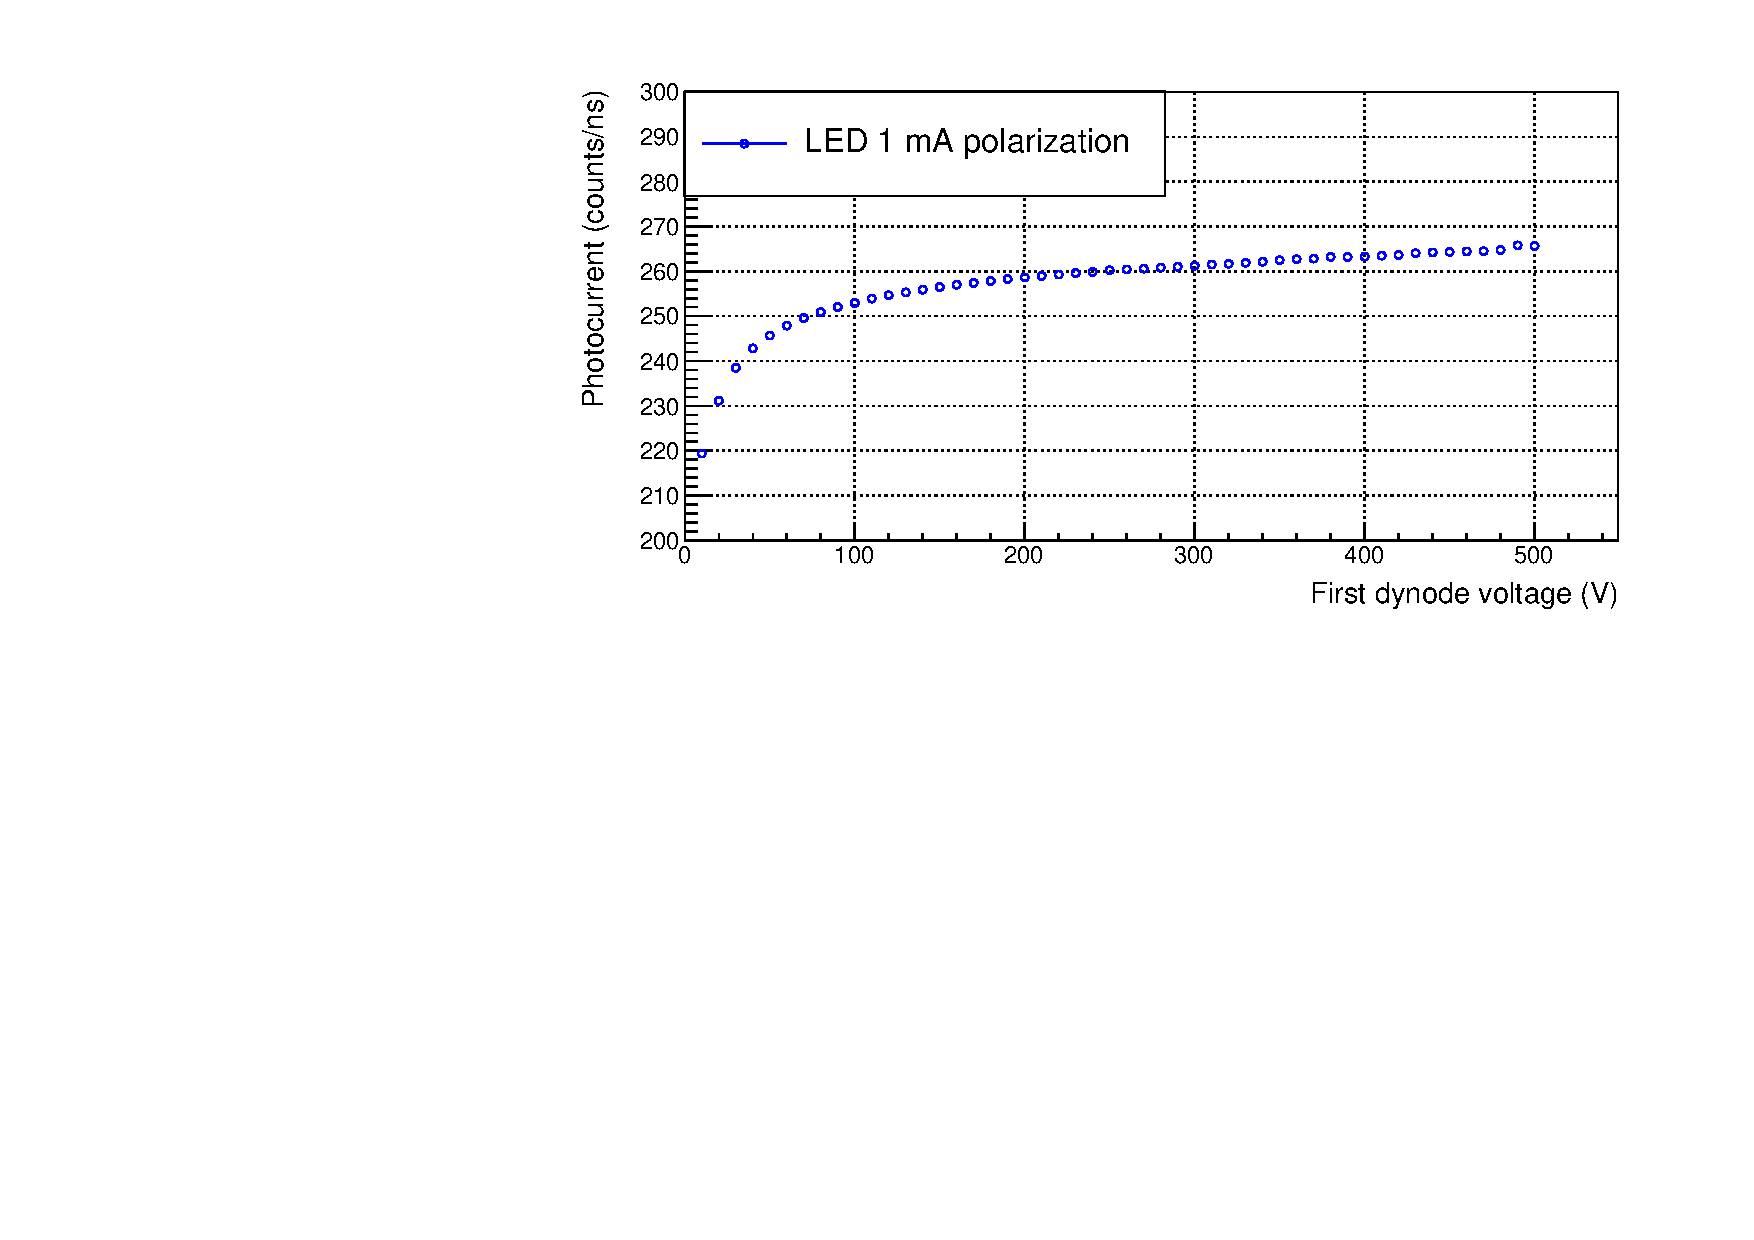
\includegraphics[scale=0.7]{4ResearchAndDevelopments/41Fibers/PCBNoGainPlateau_Calibrated.pdf}
\caption{PMT photocurrent as a function of the first dynode voltage with the dark current subtracted. Error bars are smaller than dot size.\label{fig:PlateauNoGainPMT}}
\end{figure}

The linear response of the PMT (in absence of fibres) was verified in two different ranges, $[0-30]~\text{photons}/\nano\second$ which is the expected number of photons for tritium events, and $[0-2500]~\text{photons}/\nano\second$, employed for fibre characterization. The results for the low and high illumination cases are plotted in Figure \ref{fig:LinearityRangesOfPMT}. No saturation of the PMT response is observed.

\begin{figure}
\centering
    \begin{subfigure}[b]{1\textwidth}
    \centering
    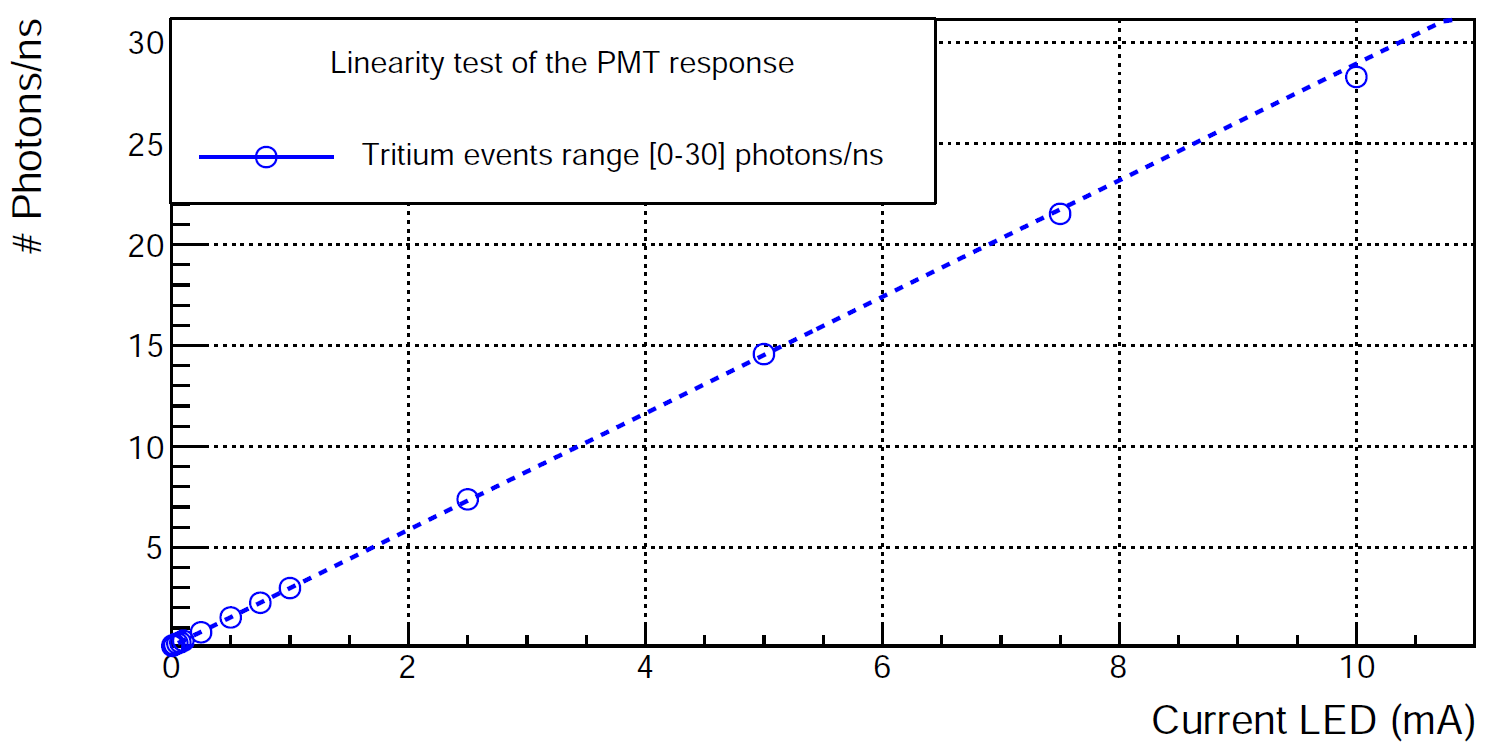
\includegraphics[scale=0.4,width=\textwidth]{4ResearchAndDevelopments/41Fibers/Linearity_test_0_30_range.png}  
    \caption{\label{subfig:LinearityTritiumRange}}
    \end{subfigure}
    \hfill
    \begin{subfigure}[b]{1\textwidth}
    \centering
    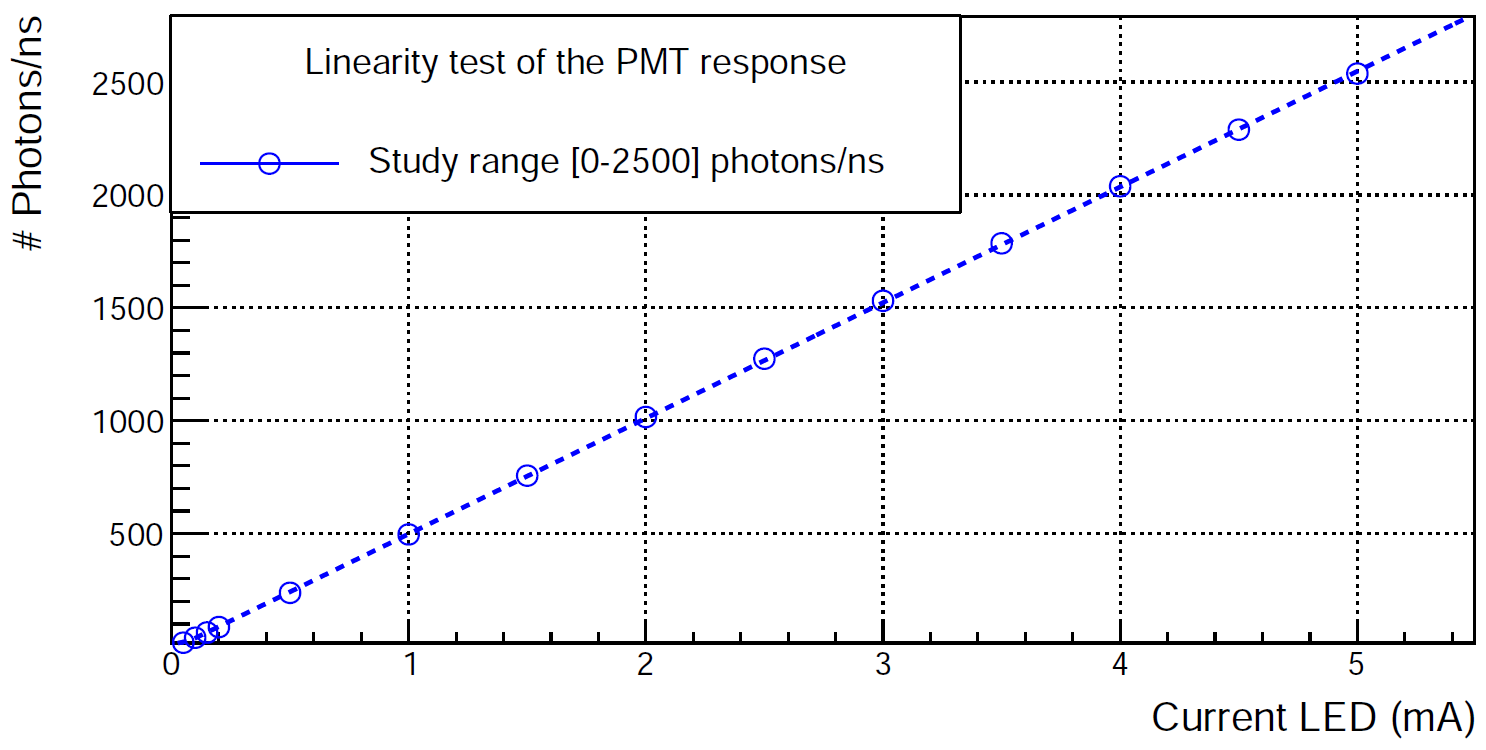
\includegraphics[scale=0.4, width=\textwidth]{4ResearchAndDevelopments/41Fibers/Linearity_test_0_2500_range.png}  
    \caption{\label{subfig:LinearityStudyRange}}
    \end{subfigure}
 \caption{Rate of photons measured by the PMT as a function of the LED current. a) Response of the PMT in the intensity range of tritium events. b) Response of the PMT in the range $0-2500~\text{photons}/\nano\second$. Error bars are smaller than the dot size.}
 \label{fig:LinearityRangesOfPMT}
\end{figure}